\chapter{Results}


\section{Naive Bayes Evaluation}

Before evaluating the application of the Naive Bayes classifier in the chess engine, it is important to evaluate the classifier on its own. A total of 12 models were trained, including 3 different datasets and 4 different feature sets (labelled 0 to 3). Each model was trained on 300,000 games from the Lichess database. The results are summarised in Table \ref{tab:naive_bayes_evaluation}.

% Dataset,model,f1,kappa,accuracy,recall,precision
% master,0,0.5988536304236853,0.2112254147134801,0.6049062609492699,0.482094782209774,0.6439416616022197
% beginner,0,0.6051249676934042,0.2210397399646341,0.609488133601887,0.5040674214143965,0.6466855707935595
% random,0,0.6072031151366292,0.22365713746617322,0.6107085997032513,0.5156335065526249,0.646008464803797
% master,1,0.605130502829087,0.21395189271532478,0.6066231824687036,0.5446936268591849,0.6257603246825858
% beginner,1,0.6099898344486384,0.22289154075242434,0.610955667581852,0.5600284176270772,0.630317464411715
% random,1,0.6113403483186637,0.22495286229881817,0.6119870906691742,0.569425141503181,0.6304191915229441
% master,2,0.6085085653811569,0.21817535774911112,0.6089051908184601,0.5763088238844891,0.6202536271310867
% beginner,2,0.6112343011853606,0.22422735972358465,0.611752390275514,0.5737754871653842,0.6274838694106847
% random,2,0.6130669539707349,0.22692003179415388,0.6132139510830144,0.590906779230026,0.6260967043218012
% master,3,0.6084997597868439,0.2172749652323428,0.6085624145434425,0.5947075103824608,0.6152391256154944
% beginner,3,0.61155981712515,0.22315316162034304,0.6115478379550269,0.6072561711576363,0.6185306574839604
% random,3,0.6124781405192362,0.2248037693959768,0.6124678472852909,0.6162927292084742,0.6187451294855816


\begin{table}[H]
    \centering
    \begin{tabular}{|c|c|c|c|c|c|c|}
    \hline
    \textbf{Dataset} & \textbf{Model} & \textbf{F1 Score} & \textbf{Kappa Score} & \textbf{Accuracy} & \textbf{Recall} & \textbf{Precision} \\ \hline
    Master           & 0              & 0.5989            & 0.2112              & 0.6049            & 0.4821         & 0.6439            \\ \hline
    Beginner         & 0              & 0.6051            & 0.2210              & 0.6095            & 0.5041         & 0.6467            \\ \hline
    Random           & 0              & 0.6072            & 0.2237              & 0.6107            & 0.5156         & 0.6460            \\ \hline
    Master           & 1              & 0.6051            & 0.2139              & 0.6066            & 0.5447         & 0.6258            \\ \hline
    Beginner         & 1              & 0.6100            & 0.2229              & 0.6110            & 0.5600         & 0.6303            \\ \hline
    Random           & 1              & 0.6113            & 0.2249              & 0.6120            & 0.5694         & 0.6304            \\ \hline
    Master           & 2              & 0.6085            & 0.2182              & 0.6089            & 0.5763         & 0.6203            \\ \hline
    Beginner         & 2              & 0.6112            & 0.2242              & 0.6118            & 0.5738         & 0.6275            \\ \hline
    Random           & 2              & 0.6131            & 0.2269              & 0.6132            & 0.5909         & 0.6261            \\ \hline
    Master           & 3              & 0.6085            & 0.2173              & 0.6086            & 0.5947         & 0.6152            \\ \hline
    Beginner         & 3              & 0.6116            & 0.2232              & 0.6115            & 0.6073         & 0.6185            \\ \hline
    Random           & 3              & 0.6125            & 0.2248              & 0.6125            & 0.6163         & 0.6187            \\ \hline
    \end{tabular}
    \caption{Naive Bayes Evaluation}
    \label{tab:naive_bayes_evaluation}
\end{table}


The average F1 value overall was 0.608 across the 12 different models. This shows that the classifier was able to learn some aspects of the game, however despite this, considering a random classifier would have an F1 score of 0.5, an F1 score of 0.608 is not very good. This is further supported by the Kappa score which averaged 0.221. This would come under the category of "fair agreement" according to Landis and Koch \cite{landisMeasurementObserverAgreement1977}, demonstrating that the classifier was able to understand some indicators of winning or losing positions. However the low Kappa and F1 scores reinforce the known limitations of Naive Bayes, particularly its reliance in the assumption of conditional independence. The models were not able to learn the complex relationships between the features and the result of the game, which is crucial in chess. This indicates that Naive Bayes is not suitable for applications where the results are highly dependent on feature interactions. An average accuracy of 0.610 highlights the model's ability to learn some patterns in the data. Precision is important in the context of chess since it reflects how often the model's predicted winning outcomes are correct. A low precision would mean the model may not consider safer moves, being led to make riskier decisions. A precision of 0.620 was obtained indicating the model's ability to identify winning positions. Recall is another important measure to consider in the context of chess. It reflects the the proportion of actual winning positions that were correctly identified by the model. A low recall could cause the engine to miss critical chances to press an advantage. The average recall was 0.561, indicating the model's poor ability to identify a good number of winning positions. 

Another important aspect that is important to analyse is the influence of the feature selection on the performance of the model. Across the 12 models, the progression from feature set 0 and feature set 3 showed an increase in both F1 and recall. The average F1 score for feature set 0 was 0.604 increasing to 0.622 with feature set 3, reflecting a clear trend that more features yield better performance. This is consistent with the literature, like mentioned by Sahami et al. \cite{sahamiBayesianApproachFiltering} where the addition of hand-crafted features led to significant improvement,  and Rish on his analysis on Naive Bayes \cite{rishEmpiricalStudyNaive}. The average of recall from 0.500 to 0.618 also indicates the model's ability to identify winning positions improved with the addition of more features. This is an important result as it suggests that reliance on simplistic indicators like material balance and mobility alone is not sufficient to capture the complexity of chess. Another notable observation is the minimal performance difference between feature sets 2 and 3. Both feature sets obtained a F1 score of 0.612. This plateau indicates possible diminishing returns with the addition of more features. One possible explanation for this is that the added features, like king safety and castling rights, may be strongly correlated to existing features, leading to minimal information gain. Another explanation to this is that the model did not see enough examples of these features in play in the training data to learn their significance. These findings further reinforce that the performance of the Naive Bayes Classifier is not only dependent on the quantity of features but also on the quality of the features. The results also indicate that Naive Bayes may be limited in this context as the performance seems to reach a limit despite the increase in features and feature complexity, where more complex models may succeed. The small increase in feature set 2 and 3 could also imply that most of the useful information that the model uses for its predictions is from previous features like control of centre and pawn structure, this observation would not have been possible with a machine learning technique that is not interpretable like a neural network. 


In addition to feature selection, the dataset used to train the model has a noticeable impact on the predictive power of the classifier. What was interesting from this data, is that across all feature sets, the models trained on the random dataset consistently outperformed the models trained on the beginner and master datasets. This trend was shown by the F1 score and accuracy where, the random dataset obtained the highest f1 and accuracy scores, with an average of 0.611 and 0.612 respectively. Whereas the master dataset obtained the lowest f1 and accuracy scores, with an average 0.605 and 0.607 respectively. This result is surprising as what would be expected is that the master dataset would be more informative of good moves and winning positions. There are a number of reasons this result could have occurred. These results could be due to the nature of games in each dataset. In master-level games, there tend to be more complex positions and strategies, including more subtle positional considerations and more long term sacrificing and planning, which are difficult to learn in a probabilistic model like Naive Bayes. These complex reasonings for each move violate the assumption of feature independence, resulting in poorer generalisation. This is in contrast to the random dataset which would include a more variety of playing styles and patterns, which could be based on more straightforward principles like material balance which Naive Bayes can detect with better accuracy.


\section{MMNB Analysis}

To evaluate the performance of Naive Bayes in a minimax algorithm, two versions were compared. The first being MMNB integration which combines the Naive Bayes evaluation with a traditional evaluation function, and the second being MMNB substitution which completely replaces the evaluation function in the minimax algorithm. Several performance indicators were used to analyse the 2800 games played including mobility, blunder frequency and stockfish evaluations. These indicators provide a comprehensive understanding of the engine's ability in making strategic decisions by both implementations.


The results between MMNB integration and MMNB substitution, reveal a much stronger performance from the MMNB integration. This is supported by the graph in Figure \ref{fig: implementation_vs_win_rate} as well as the raw values obtained.

\begin{figure}[H]
    \centering
    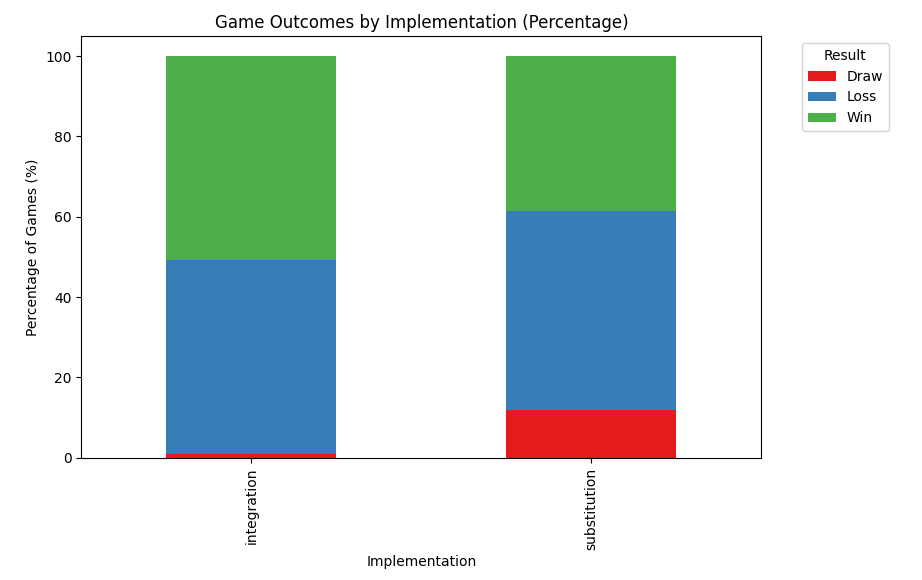
\includegraphics[width=0.8\textwidth]{images/plots/implementation/Implementation_vs_win_rate.png}
    \caption{Game Outcomes of each Implementation}
    \label{fig: implementation_vs_win_rate}
\end{figure}


% ======================================================================  
% OVERALL WIN/DRAW/LOSS RATES BY IMPLEMENTATION
% ======================================================================  
% integration (Total games: 8634):
%   Win:  4378 games (50.7%)
%   Draw: 84 games (1.0%)
%   Loss: 4172 games (48.3%)

% substitution (Total games: 3840):
%   Win:  1484 games (38.6%)
%   Draw: 460 games (12.0%)
%   Loss: 1896 games (49.4%)


% ======================================================================  
% WIN/DRAW/LOSS RATES BY IMPLEMENTATION AND OPPONENT
% ======================================================================  

% Opponent: random
% --------------------------------------------------
% integration (Total games: 4314):
%   Win:  4290 games (99.4%)
%   Draw: 24 games (0.6%)
%   Loss: 0 games (0%)

% substitution (Total games: 1920):
%   Win:  1484 games (77.3%)
%   Draw: 436 games (22.7%)
%   Loss: 0 games (0%)


% Opponent: stockfish
% --------------------------------------------------
% integration (Total games: 4320):
%   Win:  88 games (2.0%)
%   Draw: 60 games (1.4%)
%   Loss: 4172 games (96.6%)

% substitution (Total games: 1920):
%   Win:  0 games (0%)
%   Draw: 24 games (1.2%)
%   Loss: 1896 games (98.8%)


The integration implementation achieved a win rate of 50.7\%, with loses at 48.3\% and draws only at 1.0\%. In contrast, the substitution implementation achieved a win rate of 38.6\%, a similar loss rate of 49.4\% and a much higher draw rate of 12.0\%. This notable difference in draw rates suggests that MMNB substitution wasn't able to identify moves that would lead to wins even when in advantageous positions or the inability to identify crucial moves. 

It is important to seek deeper insight into this pattern by comparing the results of the two implementations against both opponents, Stockfish and random engine. Against the random opponent, MMNB integration dominated, winning 99.4\% of the games and never losing. MMNB substitution, however, did do well but achieved a much lower win rate of 77.3\% and a much higher draw rate of 22.7\%. This contrast of win rates, indicate that even against a low-skill opponent, with no strategy, the substitution engine was much worse at converting advantages into wins.

This is further supported by the games against Stockfish. MMNB integration was able to win 2.0\% of the games and draw 1.4\% of games whereas MMNB substitution failed to win even a single game, drawing only 1.2\% of the time and losing 98.8\% of the games. This highlights the limitation of the substitution implementation which is the evaluation function. The evaluation function which solely relies on the Naive Bayes probabilities, does not have the necessary understanding to win against a strong opponent. Despite being outperformed by Stockfish, the integration method showed that ability to exploit certain rare strategic opportunities, which is likely only due to the hybrid approach. These findings reinforce the hypothesis that Naive Bayes is best used as a supporting tool in a chess engine. The simplicity of the Naive Bayes classifier can provide some useful insights but is insufficient to be used as a standalone evaluation function.

Figure \ref{fig: implementation_vs_win_rate} is a good indicator of the overall performance of both engines but does not provide an insight of the quality of moves and efficiency of the engines. One way to measure the quality of moves is to compare the stockfish evaluation after each move as well as the average value of the blunders made by each engine. The results are shown in Figure \ref{fig: implementation_vs_stockfish_eval_and_blunder_value}.

\begin{figure}[H]
    \centering
    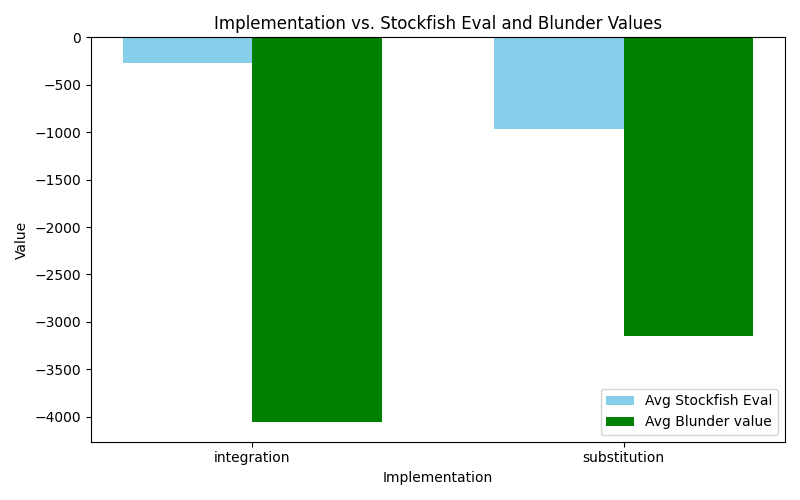
\includegraphics[width=0.8\textwidth]{images/plots/implementation/Implementation_vs_stockfish_eval_and_blunder_value.png}
    \caption{Stockfish Evaluation and Blunder Value of each Implementation}
    \label{fig: implementation_vs_stockfish_eval_and_blunder_value}
\end{figure}

% ======================================================================  
% AVERAGE STOCKFISH EVALUATION BY IMPLEMENTATION
% ======================================================================  
% integration: -340.02

%   By opponent:
%     vs random: 2241.98
%     vs stockfish: -2918.43

% substitution: -1048.25

%   By opponent:
%     vs random: 1099.23
%     vs stockfish: -3195.74

% ======================================================================
% AVERAGE BLUNDER SEVERITY BY IMPLEMENTATION (ONLY NON-ZERO BLUNDERS)
% ======================================================================
% integration: -4693.34 (13690 blunders)

%   By opponent:
%     vs random: -4617.38 (6200 blunders)
%     vs stockfish: -4756.22 (7490 blunders)

% substitution: -2652.59 (34364 blunders)

%   By opponent:
%     vs random: -2423.47 (30988 blunders)
%     vs stockfish: -4755.65 (3376 blunders)


The Stockfish evaluation is a numerical representation of the the move quality, where a higher value indicates a better move. Figure \ref{fig: implementation_vs_stockfish_eval_and_blunder_value} that the MMNB integration engine had a higher average stockfish evaluation than the MMNB substitution engine, which is consistent with the conclusions obtained based on the win rates. MMNB integration had an average stockfish evaluation of -340.02, whereas MMNB substitution had an average stockfish evaluation of -1048.25. However what is interesting is the average blunder value of each implementation. A blunder was defined as a move that caused a decrease in the Stockfish evalutaion by 300, where a more negative value indicates a more severe blunder based on Stockfish's opinion. MMNB integration had an average blunder value of -4693.34, whereas MMNB substitution had an average blunder value of -2652.59. This suggests that even though MMNB integration was able to win more games, it made more severe blunders. This could suggest that the integration method played much more aggressive and making more risky moves. This would explain the higher win rate but also the much higher average blunder value. Whereas the substitution engine played much more conservatively and avoided making more riskier moves, which is why it had a lower win rate since it was unable to exploit certain opportunities. 

% ======================================================================
% AVERAGE NUMBER OF NON-ZERO BLUNDERS PER WHOLE GAME BY IMPLEMENTATION
% ======================================================================
% integration (2160 games): 3.17 non-zero blunders per game

%   By opponent:
%     vs random (1080 games): 2.87 non-zero blunders per game
%     vs stockfish (1080 games): 3.47 non-zero blunders per game

% substitution (960 games): 17.90 non-zero blunders per game

%   By opponent:
%     vs random (480 games): 32.28 non-zero blunders per game
%     vs stockfish (480 games): 3.52 non-zero blunders per game

As much as blunder value indicates that integration caused much more severe blunders, it is also important to consider the average number of blunders made by each implementation. Despite the average blunder value being lower for the substitution implementation, it made over 6 times more blunders per game than the integration implementation. MMNB integration had an average of 3.17 blunders per game whereas MMNB substitution had an average of 17.90 blunders per game. This shows that the substitution implementation was much more prone to blunders, despite having a much lower average blunder value. This further 
confirms the theory that solely basing the evaluation function on the Naive Bayes classifier is detrimental to the engine's performance whereas a an approach that combines traditional methods and Naive Bayes can be much more fruitful.


Two good indicators of the performance of the engines during different phases of the game, is mobility and piece balance. Piece balance meaning the difference in material between both players and mobility referring to the number of possible moves the player can make. Figure \ref{fig: implementation_vs_avg_piece_balance_and_phase } and \ref{fig: implementation_vs_avg_mobility_and_phase} show the average piece balance and mobility of each implementation over different phases of the game. The opening phase was defined by the first 25\% of the game, midgame phase was defined by the next 50\% of the game and endgame was defined by the last 25\% of the game.

\begin{figure}[H]
    \centering
    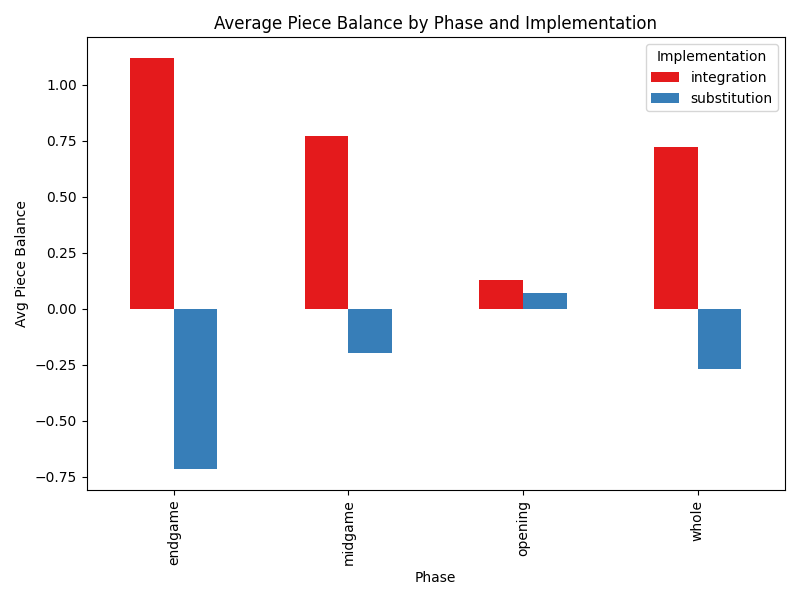
\includegraphics[width=0.8\textwidth]{images/plots/implementation/Implementation_vs_avg_piece_balance_and_phase.png}
    \caption{Average Piece Balance per Game of each Implementation}
    \label{fig: implementation_vs_avg_piece_balance_and_phase }
\end{figure}




% ======================================================================
% AVERAGE PIECE BALANCE BY PHASE AND IMPLEMENTATION  
% ======================================================================
% implementation  integration  substitution
% phase
% endgame            1.119188     -0.716872
% midgame            0.769215     -0.198002
% opening            0.126352      0.071598
% whole              0.722590     -0.267395

Figure \ref{fig: implementation_vs_avg_piece_balance_and_phase } shows that the integration method always had a higher piece balance than the substitution method across all the different game phases. MMNB integration achieved an average piece balance of 0.723, indicating the engine's understanding of the importance of having material advantage over the opponent. On the other hand, MMNB substitution has an average piece balance of -0.267, indicating that the engine was often at a material disadvantage. The integration implementation consistently outperformed the substitution implementation in piece balance across all game phases. Both implementations, in the opening phase, had similar positive piece balances indicating their understanding of the importance of material advantage. However during midgame and end game, MMNB integration considerably outperformed the substitution implementation, achieving an average piece balance of 0.769 and 1.119 respectively, whereas the substitution implementation had an average piece balance of -0.198 and -0.716 respectively. This highlights the integration method's ability to preserve and accumulate material advantage, across different stages. These observations suggest that combining Naive Bayes with a classical evaluation function supports better piece management and leads to fewer unfavourable trades. Conversely, reliance purely on Naive Bayes 
leads to more frequent disadvantageous exchanges, decreasing overall material count over time which is critical in the midgame and endgame phases. The hybrid approach evidently takes 
advantage of core chess principles, while still benefiting from probabilistic insights, resulting in higher piece balance and overall performance.

\begin{figure}[H]
    \centering
    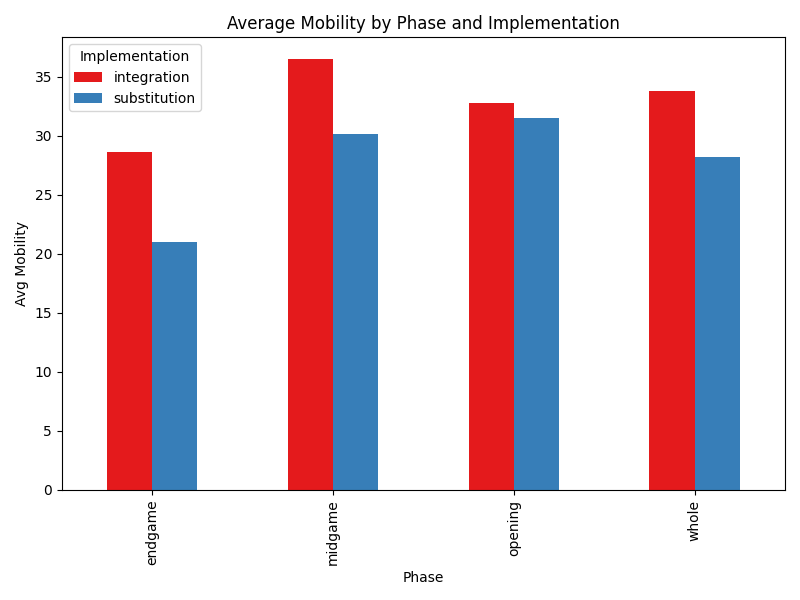
\includegraphics[width=0.8\textwidth]{images/plots/implementation/Implementation_vs_avg_mobility_and_phase.png}
    \caption{Average Mobility per Game of each Implementation}
    \label{fig: implementation_vs_avg_mobility_and_phase}
\end{figure}

% ======================================================================
% AVERAGE MOBILITY BY PHASE AND IMPLEMENTATION       
% ======================================================================
% implementation  integration  substitution
% phase
% endgame           28.583730     21.022493
% midgame           36.500683     30.159101
% opening           32.733946     31.481510
% whole             33.752626     28.199893


Mobility is measured by the average number of legal moves available at each turn. In chess theory, a higher mobility correlates with better board control, increasing tactical opportunities. Again, the integration method consistently surpassed the substitution method in mobility across all game phases. 
Overall, MMNB integration achieved an average mobility of 33.75 whereas MMNB substitution achieved an average mobility of 28.20, a gap of about 5.55 moves. In the opening, the average mobility is very similar inidicating similar strategies by both implementations. However, in midgame, where there is more complexity and opportunities since there are still a lot of pieces but are more developed. Integration has a higher mobility by about 6.34 moves (36.50 vs 30.16). This result was further amplified in the endgame where integration had an average mobility of 28.58 compared to 21.02 of the substitution implementation, a difference of 7.56 moves. Endgames require more precise and calculated moves minimising mistakes. This difference between the two indicates that MMNB substitution often causes pieces to move into more restricted or disadvantageous positions, while integration retains better piece coordination and mobility. There are a number of points that can be learnt from these results. Firstly, the integration method's superior mobility suggests it aims to avoid cramped locations and favour open positions, which is crucial throughout the game. MMNB substitution is strictly relying upon the assumption of feature independence. In the domain of chess where all features of the game are interdependent, it can lead to suboptimal decisions. The integration method's ability to combine the strengths of both Naive Bayes and traditional evaluation functions allows it to better navigate the complexities of chess, leading to improved mobility. These findings corroborate what has been concluded from previous metric results, indicating that pure Naive Bayes is less effective in understanding the nuances of the board while a hybrid approach preserves strategic principles and enhances mobility.

So far what has been assessed between the two implementations is different metrics to assess the performance of the engine. Another factor that is important to consider is the the time taken to make each move as if it is to be used in real time, it is important that it is able to make decisions in a reasonable time period. Figure \ref{fig: implementation_vs_avg_move_time_and_phase} shows the average time taken to make each move across the different phases of the game.

\begin{figure}[H]
    \centering
    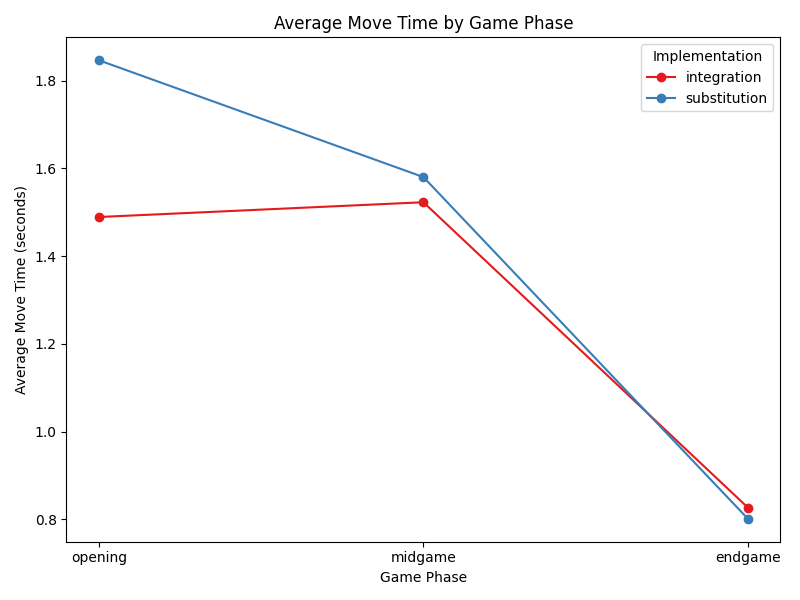
\includegraphics[width=0.8\textwidth]{images/plots/implementation/Implementation_vs_avg_move_time_and_phase.png}
    \caption{Average Time Taken to Make Each Move of each Implementation}
    \label{fig: implementation_vs_avg_move_time_and_phase}
\end{figure}

% Average Move Time by Phase and Implementation:
%      phase implementation  avg_move_times
% 0  opening    integration        1.489163
% 1  opening   substitution        1.846336
% 2  midgame    integration        1.522826
% 3  midgame   substitution        1.580211
% 4  endgame    integration        0.827023
% 5  endgame   substitution        0.801537
% 6    whole    integration        1.334166
% 7    whole   substitution        1.444066

The horizontal x-axis shows reflects the different phases of the game. The overall average time taken to make a move for MMNB integration was 1.334 seconds in comparison to 1.444 seconds for MMNB substitution. This indicates the integration method was able to make decisions faster than the substitution method. This is an important result as it hightlights that MMNB integration is not only more effective in winning games but also is more efficient in making decisions. In the opening phase, substitution has the longest move time at 1.846 seconds, which is 0.36 seconds longer than integration. This suggests that the pure Naive Bayes evaluation requires more computational effort or more likely, struggles to prune effectively early on. This is likely due to the fact that the opening phase there are many more pieces so a lot more possible moves, requiring more time to evaluate moves. In midgame the overall time taken to make a move decreases in both methods to 1.522 seconds for integration and 1.580 seconds for substitution. During the midgame phase, the complexity of the game increases however the overall number of pieces on the board decreases, which would require less time to evaluate moves. In the endgame phase, both engines drop below 1 second, with integration taking 0.827 seconds and substitution taking 0.801 seconds. This is expected as during endgame there are much less pieces on the board, reducing the branching factor of the search tree. Substitution is slightly faster than integration in the endgame phase,  but this is most likely due to what was discussed earlier and that substitution on average has less material on the board, resulting in less possible moves, requiring less time to evaluate. In the openinng and midgame phases, the substitution method seems to either take longer to evaluate moves or is less efficient in pruning the search tree. As the game progresses, there are less pieces and opportunities to make moves, narrowing the difference between the two implementations. Another important observation to note is the efficiency vs. effectiveness of the two implementations. Generally, an increase in one, causes a decrease in the other however the data shows otherwise. While substitution invests more time in evaluating moves, it is still not able to outperform integration, suggesting that longer computation time doesn't necessarily result in better moves. 

\begin{figure}[H]
    \centering
    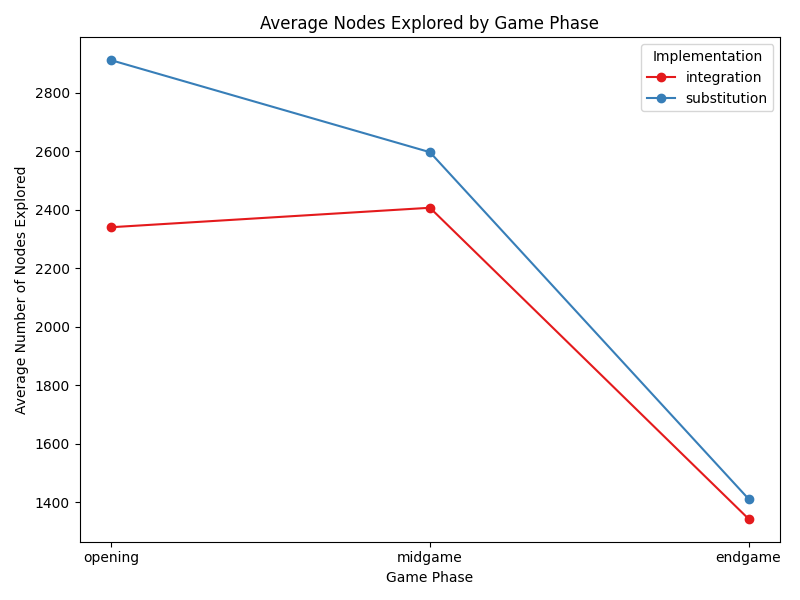
\includegraphics[width=0.8\textwidth]{images/plots/implementation/Implementation_vs_avg_nodes_explored_and_phase.png}
    \caption{Average Nodes Explored per Game of each Implementation}
    \label{fig: implementation_vs_avg_nodes_explored_and_phase}
\end{figure}

% Average Nodes Explored by Phase and Implementation:
%      phase implementation  avg_nodes_explored
% 0  opening    integration         2339.930400
% 1  opening   substitution         2910.269032
% 2  midgame    integration         2406.379927
% 3  midgame   substitution         2596.181826
% 4  endgame    integration         1343.829285
% 5  endgame   substitution         1411.950722
% 6    whole    integration         2114.515511
% 7    whole   substitution         2366.398302

Figure \ref{fig: implementation_vs_avg_nodes_explored_and_phase} shows the average number of nodes evaluated during the search of the game trees. The general trend is that the average number of nodes explored decreases as the game progresses. Similar to average time taken to make a move, this is expected as the number of pieces on the board decreases, reducing the branching factor of the search tree. The average number of nodes explored by MMNB integration was 2115 whereas the average number of nodes explored by MMNB substitution was 2366. In the opening phase, substitution explored 2910 nodes on average compared to 2339 for integration. This difference of 571 nodes indicates that the substitution method was less efficient in pruning the search tree, affirming the earlier observation that substitution takes longer to evaluate moves. The number of nodes explored closer to endgame is much closer between the two implementations. These results point towards the success of the hybrid approach in effectively pruning the search tree, leading to a more efficient evaluation process due ot the insight it gains from both the Naive Bayes classifier and the traditional evaluation function. 

These two figures show that MMNB substitution contiuously spends more time and searches more nodes in early phases of the game but despite this still fails to yield better results than MMNB integration. This pattern reinforces that combining Naive Bates with standard heuristics genreally results a more efficient and reliable approach to the minimax search over exclusively relying on Naive Bayes, particularly during opening phases.


\section{Feature Selection Analysis}

The feature sets were designed to be progressively more complex, with the aim of evaluating the impact of feature selection on the performance of the Naive Bayes classifier. The results from the previous section show that the addition of more features generally leads to better performance. However it is also important to see their impact on the gameplay of the engine. Figure \ref{fig: feature_set_vs_win_rate} shows the overall performance of each feature set in terms of wins, draws and losses.
\begin{figure}[H]
    \centering
    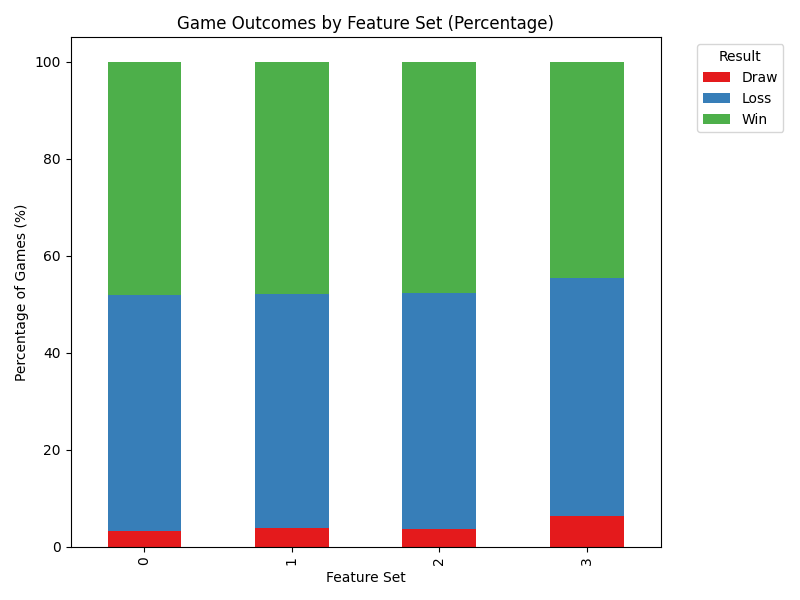
\includegraphics[width=0.8\textwidth]{images/plots/featureSet/Feature_set_vs_win_rate.png}
    \caption{Game Outcomes of each Feature Set}
    \label{fig: feature_set_vs_win_rate}
\end{figure}



% Feature Set 0:
%   Draw: 3.3%
%   Loss: 48.6%
%   Win: 48.1%
%   (Total games: 3360)

% Feature Set 1:
%   Draw: 3.9%
%   Loss: 48.2%
%   Win: 47.9%
%   (Total games: 2874)

% Feature Set 2:
%   Draw: 3.6%
%   Loss: 48.8%
%   Win: 47.6%
%   (Total games: 2880)

% Feature Set 3:
%   Draw: 6.4%
%   Loss: 49.0%
%   Win: 44.5%
%   (Total games: 3360)




Overall the different feature sets showed a similar trend in performance. Feature sets 0, 1 and 2 had win rates around 48\%, loss rates around 48\% to 49\% and draw raters around 3\% to 4\%. However, feature set 3 had a noticeable jump in draw rates to 6.4\%, nearly double the previous feature sets. It also had a noticeable decrease in win rates to 44.5\%. The increase in draw rates could suggest that the engine was more conservative in its play, staying away from riskier moves. This would also clarify the decrease in win rate since the engine was not able convert games into wins due to its defensive play. These results indicate that the addition of more features does not have a big impact on the gameplay of the engines. The similar win and loss rates across feature sets 0, 1 and 2 indicate the engine's ability to apply basic chess principles but was unable to apply the increasing complexity of the features and learn from the increased information. The sharp change in rates for feature set 3, however, indicate that the the complexity of the features may have caused the engine to become more uncertain in its moves, causing it to draw more and fail to win as much. This could be due to feature overlapping features causing the classifier to assign incorrect probabilities \cite{ahmedOkNBEnhancedOPTICS2024} or could indicate a possible overfitting of the model. These results also could show the diminishing results of adding more features. The more simpler features might have captured most of the information and the added specialised features did not increase the information gained by the model. One last point that is notable between the first 3 feature sets is that the loss rates were very similar, however there was a slight trend of decreasing win rates. Feature set 0 achieved a win rate of 48.1\%, feature set 1 achieved a win rate of 47.9\% and feature set 2 achieved a win rate of 47.6\%. This suggests that the adding of features didn't majorly affect the engine's vulnerability to losing but did add some confusion to the model, causing it to convert potential wins into draws. Overall, this data shows that adding features slightly changes teh results, it does not necessarily improve the winning ability of the engine, as would be expected. This is proven by feature set 3, which included the features of all the other feature sets and more, still had the lowest win rate and highest draw and loss rate. This indicates that the underlying assumption of feature independence in Naive Bayes struggles to handle the interactions between a large number of chess features. Thus concluding more features doe not necessarily translate to better performance but rather depends on the quality of features. 

Despite the similarity in win and loss rates, figures \ref{fig: feature_set_vs_piece_balance} and \ref{fig: feature_set_vs_blunder_count_and_avg_mobility} show different metrics of each feature set.

% ======================================================================
% METRICS BY FEATURE SET
% ======================================================================
% Feature Set 0:
%   Average Piece Balance: 0.475
%   Average Mobility: 31.699
%   Average Non-zero Blunders per Game: 7.258

% Feature Set 1:
%   Average Piece Balance: 0.464
%   Average Mobility: 32.574
%   Average Non-zero Blunders per Game: 6.957

% Feature Set 2:
%   Average Piece Balance: 0.552
%   Average Mobility: 32.324
%   Average Non-zero Blunders per Game: 6.728

% Feature Set 3:
%   Average Piece Balance: 0.207
%   Average Mobility: 31.695
%   Average Non-zero Blunders per Game: 9.615



\begin{figure}[H]
    \centering
    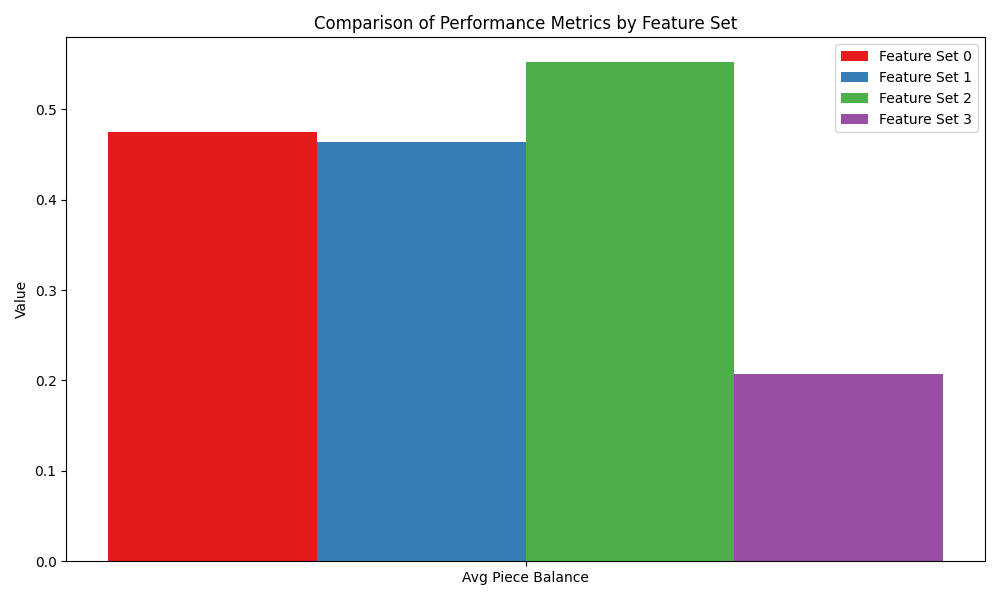
\includegraphics[width=0.8\textwidth]{images/plots/featureSet/Feature_set_vs_piece_balance.png}
    \caption{Average Piece Balance of each Feature Set}
    \label{fig: feature_set_vs_piece_balance}
\end{figure}


Figure \ref{fig: feature_set_vs_piece_balance} shows the average piece balance of each feature set. Overall, all feature sets had a positive piece balance, indicating the engine's strong understanding in the importance of material balance. All of the feature sets included material balance as a feature. Feature 2 stands out in the data, achieving an average piece balance of 0.552, 0.345 pieces higher than the lowest. Indicating its ability to retain more material or gain more material across the game. This feature set included pawn structure as a feature which proves the importance of pawn structure in chess and the impact it can have on the overall material balance of the game. Feature Set 3, surprisingly, again ranked the lowest with an average piece balance of 0.207. The additional complex features did not lead to improved material balance but rather made it significantly worse than the other feature sets. 


\begin{figure}[H]
    \centering
    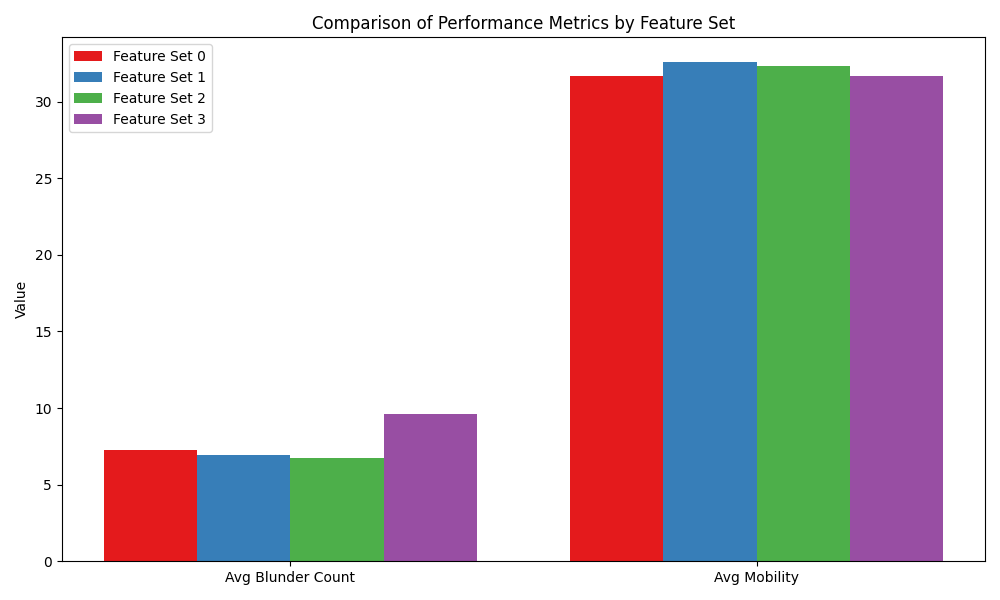
\includegraphics[width=0.8\textwidth]{images/plots/featureSet/Feature_set_vs_blunder_count_and_avg_mobility.png}
    \caption{Average Blunder Count and Mobility of each Feature Set}
    \label{fig: feature_set_vs_blunder_count_and_avg_mobility}
\end{figure}

Figure \ref{fig: feature_set_vs_blunder_count_and_avg_mobility} shows the average number of blunders made by each feature set per game. The general trend indicates the increase in features used, decreases the overall number of blunders made. Feature set 0 obtained a blunder count of 7.258, and feature set 2 achieved the  lowest at 6.728. This indicates the engine's increasingly ability to avoid making more blunders as more features were used, demonstrating the models increased learning. However, feature set 3 goes against this trend, obtaining the highest number of blunders per game at 9.615. Adding the most advanced features seem to unusually increase the number of severe mistakes made by the engine. This is provides further evidence that models trained using feature set suffer from overfitting or are affected by the dependency between features. The mobility of each feature set is roughly the same, with feature set 1 achieving the highest average mobility of 32.574 and feature set 0 achieving the lowest at 31.699. Higher mobility is a good indicator of better board control, resulting in more opportunities. 

Considering both graphs, it can be concluded that the feature set with the best overall performance is feature set 2. It achieved the highest piece balance, lowest blunder count and close to best mobility. It appears to be able to balance between complexity of features and model assumptions. The pawn structures introduced in this feature set, isolated and doubled pawns, add meaningful power without overcomplicating the model which could cause it to suffer. The most important point to understand from these results is the poor performance of feature set 3. Despite adding king safety, castling rights and game phase as features, it had the lowest piece balance, highest blunder count and close to bottom mobility. This suggests that the added features either caused the model to overfit or the fact that Naive Bayes fails to handle features that may contain more complex relationships. This demonstrates the importance of feature engineering, and that the increase in number of features does not necessarily lead to better performance but rather depends on the quality of features chosen. 


Finally, it is also important to analyse the efficiency of each feature set and if there is a benefit in using more complex features. Figures \ref{fig: feature_set_vs_avg_move_time} and \ref{fig: feature_set_vs_avg_nodes_explored} show the average time taken to make each move and the average number of nodes explored to decide each move.


% Average move times by feature set:
% Feature Set 0: 1.103 seconds
% Feature Set 1: 1.216 seconds
% Feature Set 2: 1.315 seconds
% Feature Set 3: 1.673 seconds

% Average nodes explored by feature set:
% Feature Set 0: 2225 nodes
% Feature Set 1: 2175 nodes
% Feature Set 2: 2143 nodes
% Feature Set 3: 2000 nodes


\begin{figure}[H]
    \centering
    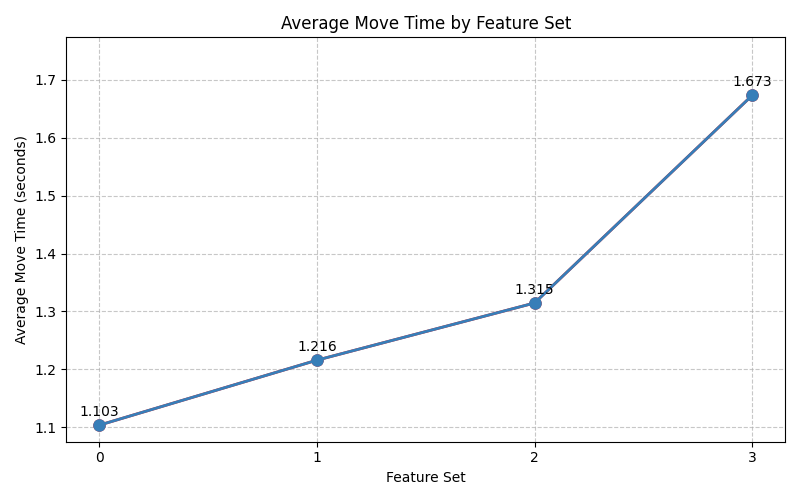
\includegraphics[width=0.8\textwidth]{images/plots/featureSet/Feature_set_vs_avg_move_time.png}
    \caption{Average Time Taken to Make Each Move of each Feature Set}
    \label{fig: feature_set_vs_avg_move_time} 
\end{figure}

Figure \ref{fig: feature_set_vs_avg_move_time} shows an overall trend of the increase in average time to make a move across the feature sets. It steadily increases from 1.103 seconds for feature set 0 to 1.315 seconds for feature set 2, which is as expected as more features are added, the model requires more time to calculate each feature, increasing the evaluation time. This is further supported by the sharp increase to 1.673 seconds for feature set 3. This is not only due to the increased number of features but also the drastic increase in the complexity of the features added. The addition of king safety, castling rights and game phase as features require much more computational effort to calculate. Even with a constant search depth, the evaluation becomes more expensive with increasing features. 


\begin{figure}[H]
    \centering
    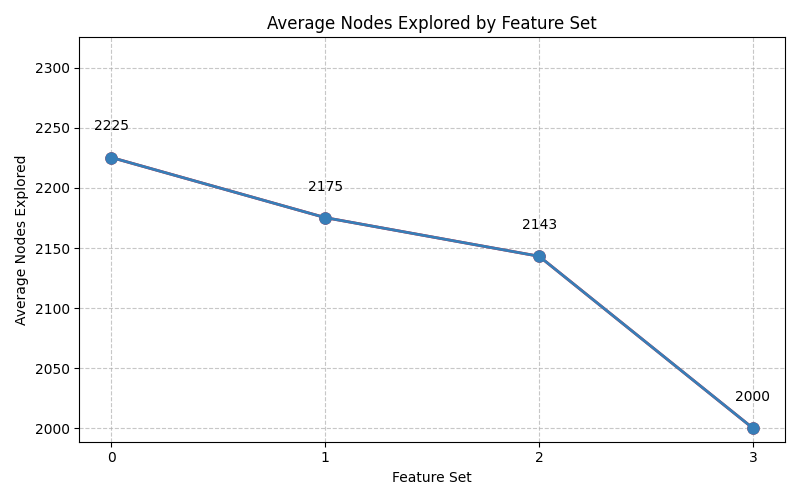
\includegraphics[width=0.8\textwidth]{images/plots/featureSet/Feature_set_vs_avg_nodes_explored.png}
    \caption{Average Nodes Explored per Game of each Feature Set}
    \label{fig: feature_set_vs_avg_nodes_explored}
\end{figure}

The general trend shown in figure \ref{fig: feature_set_vs_avg_nodes_explored} is that the average number of nodes explored decreases as the game progresses. There is a steady decrease between the first 3 feature sets from 2225 nodes for feature set 0 to 2143 nodes for feature set 2, with a more drastic decrease to 2000 nodes for feature set 3. This could suggest that the more complex features are able to prune the search tree more effectively. However, this goes against the earlier observation that the more complex features require more time to evaluate, since less nodes explored should lead to less time to decide a move. This suggests that the increase in time taken is not due to the number of nodes evaluated but rather the number of features used and the complexity of the features. 

What can be concluded from these results is that increasing the complexity of the features does  guarantee better outcomes. Despite fewer nodes being explored, the cost of evaluation increases the total move time significantly. In real-time chess engines, it is important to find a balance between a strong evaluation function and the efficiency of the evaluation. It also indicates the the additional overhead of utilising more features can be counterproductive.











